\documentclass[compress,red]{beamer}
\mode<presentation>
\setbeamertemplate{navigation symbols}{}

\usetheme{Warsaw}


%\hypersetup{pdfpagemode=FullScreen} % makes your presentation go automatically to full screen

% define your own colors:
\definecolor{Red}{rgb}{1,0,0}
\definecolor{Blue}{rgb}{0,0,1}
\definecolor{Green}{rgb}{0,1,0}
\definecolor{magenta}{rgb}{1,0,.6}
\definecolor{lightblue}{rgb}{0,.5,1}
\definecolor{lightpurple}{rgb}{.6,.4,1}
\definecolor{gold}{rgb}{.6,.5,0}
\definecolor{orange}{rgb}{1,0.4,0}
\definecolor{hotpink}{rgb}{1,0,0.5}
\definecolor{newcolor2}{rgb}{.5,.3,.5}
\definecolor{newcolor}{rgb}{0,.3,1}
\definecolor{newcolor3}{rgb}{1,0,.35}
\definecolor{darkgreen1}{rgb}{0, .35, 0}
\definecolor{darkgreen}{rgb}{0, .6, 0}
\definecolor{darkred}{rgb}{.75,0,0}

\xdefinecolor{olive}{cmyk}{0.64,0,0.95,0.4}
\xdefinecolor{purpleish}{cmyk}{0.75,0.75,0,0}


\useoutertheme[subsection=false]{smoothbars}


% include packages
\usepackage{subfigure}
\usepackage{multicol}
\usepackage{amsmath}
\usepackage{epsfig}
\usepackage{graphicx}
\usepackage[all,knot]{xy}
\xyoption{arc}
\usepackage{url}
\usepackage{multimedia}
\usepackage{hyperref}
\usepackage{helvet}
\usepackage[polish,english]{babel}
\usepackage[utf8]{inputenc}
\usepackage{multirow}
%%%%%%%%%%%%5
%\usepackage{geometry}
%\geometry{verbose,letterpaper}
%\usepackage{movie15}
%\usepackage{hyperref}
%%%%%%%

% greetings, introduce yourself


%  \includegraphics[height=5cm]{fig/WRlogo.ps}


\title[ITU-T Q13/15 meeting report\hspace{2em}\insertframenumber/\inserttotalframenumber]
{White Rabbit @ ITU-T\\ Report on Q13/15 meeting in Boulder}

\institute{
   \begin{center}
    Hardware and Timing Section\\
    CERN
   \end{center}
}
\author{
Maciej Lipi\'{n}ski %, T.W\l{}ostowski, J.Serrano, P.Alvarez
}
\date{March 2012}



% \institute%[Universities of Somewhere and Elsewhere] % (optional, but mostly needed)
% {
%   \begin{center}
%     BE-CO-HT\\
%     CERN, Geneva,\\
%     Switzerland\\
%   \end{center}
% }

\pgfdeclareimage[height=0.6cm]{wr-logo}{fig/WRlogo.ps}
\logo{\pgfuseimage{wr-logo}}
\AtBeginSection[]
% {
%   \begin{frame}<beamer>{Outline}
%     \tableofcontents[currentsection]
%   \end{frame}
% }

\begin{document}

\frame{\titlepage}
%%%%%%%%%%%%%%%%%%%%%%%%%%%%%%%%%%%%%%%%%%%%%%%%%%%%%%%%%%%%%%%%%%%%%%%%%%%%%%%%%%%%%%%%%%%%%%%%%%%%
\begin{frame}<beamer>{Outline}

    \tableofcontents %[currentsection]

\end{frame}
%%%%%%%%%%%%%%%%%%%%%%%%%%%%%%%%%%%%%%%%%%%%%%%%%%%%%%%%%%%%%%%%%%%%%%%%%%%%%%%%%%%%%%%%%%%%%%%%%%%%
\section{Introduction}
\subsection{}
%%%%%%%%%%%%%%%%%%%%%%%%%%%%%%%%%%%%%%%%%%%%%%%%%%%%%%%%%%%%%%%%%%%%%%%%%%%%%%%%%%%%%%%%%%%%%%%%%%%%
\begin{frame}{The Goal}
  
  \begin{itemize}
    \item Standardization: ultimate destination for WR
    \item ITU-T~~: Telecom PTP Profile 
    \item CERN~: White Rabbit PTP Profile 
    \item {\bf WR-PTP $\cap$ T-PTP = ?} 
  \end{itemize}

    \begin{center}
    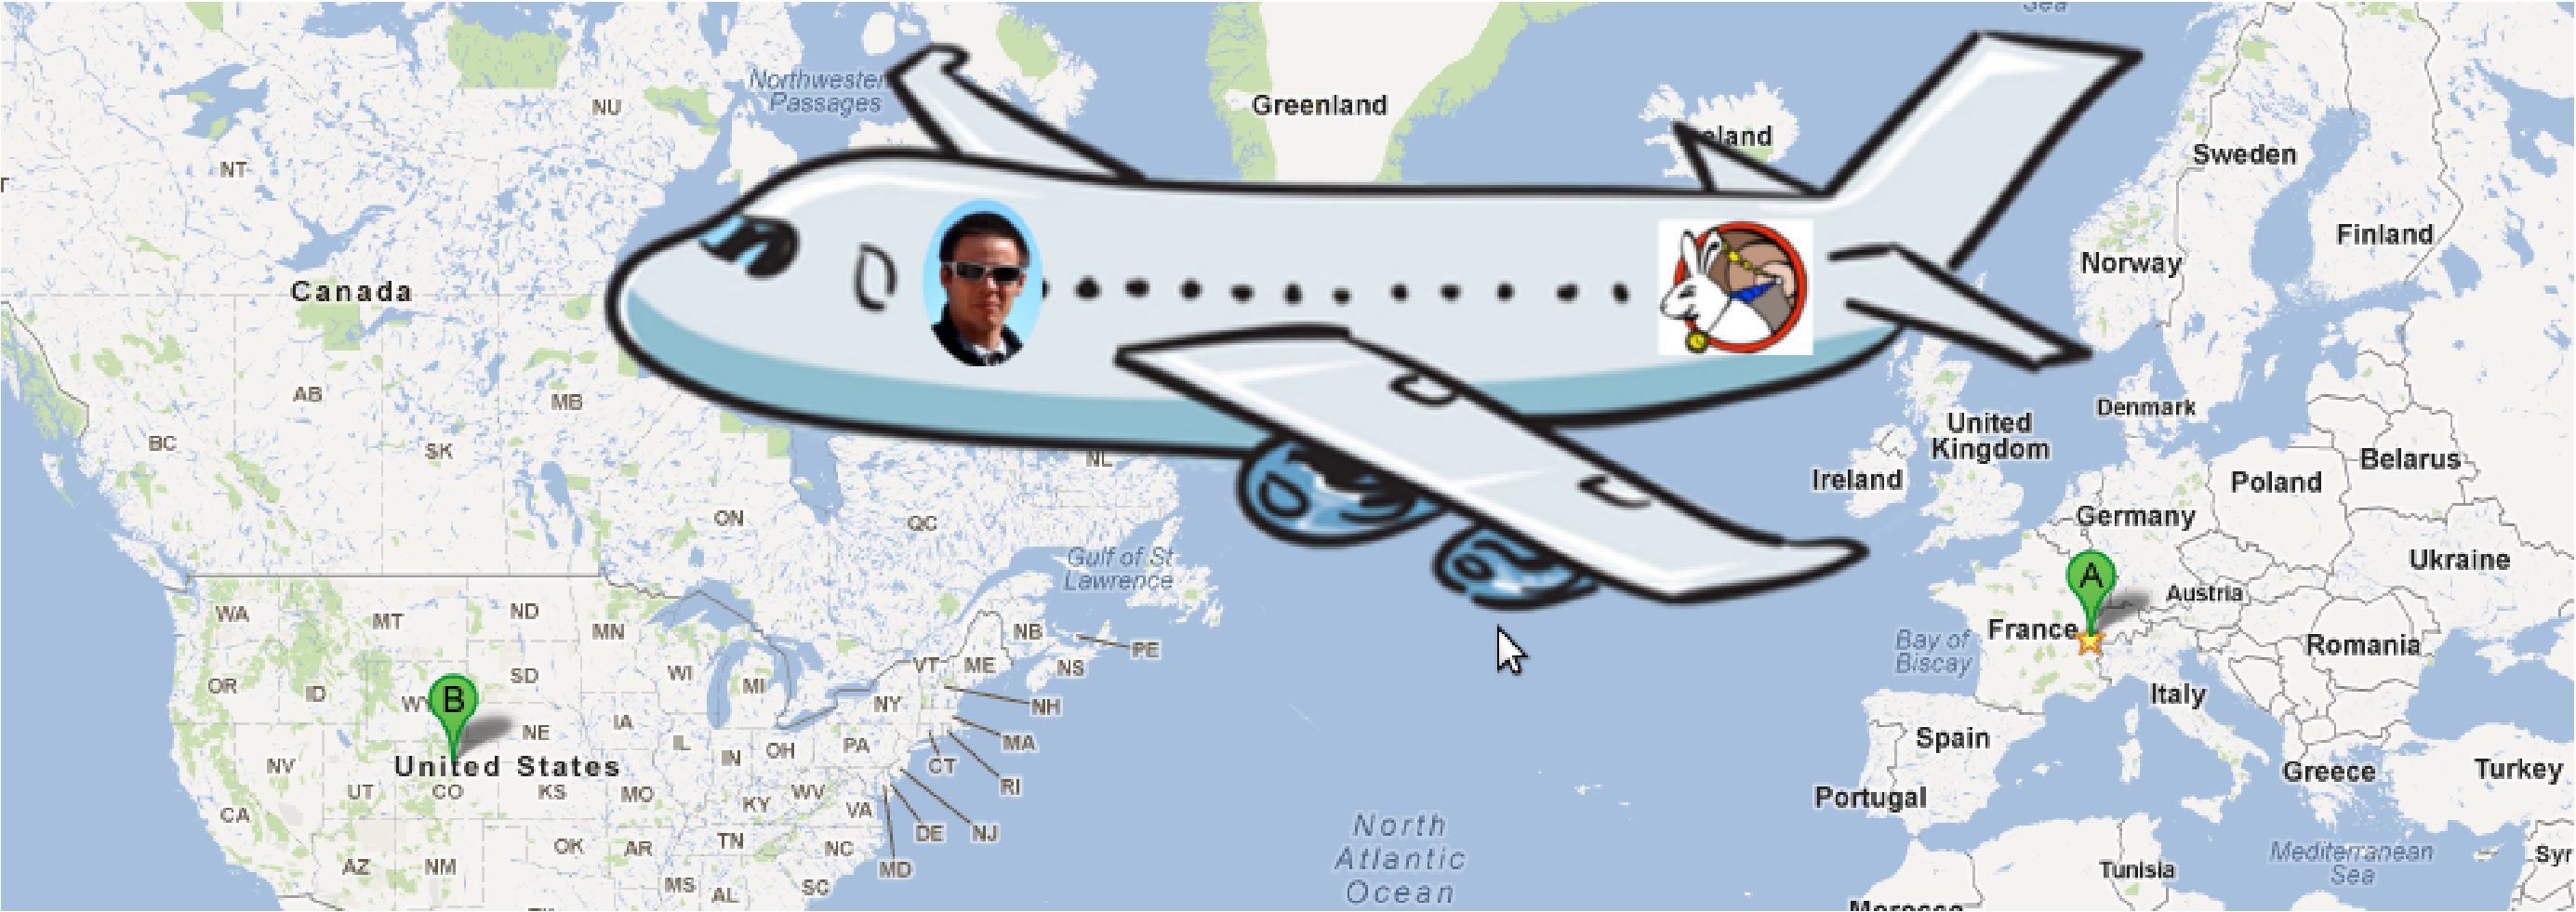
\includegraphics[height=3.5cm]{fig/gva-dva.ps}
    \end{center}


\end{frame}
%%%%%%%%%%%%%%%%%%%%%%%%%%%%%%%%%%%%%%%%%%%%%%%%%%%%%%%%%%%%%%%%%%%%%%%%%%%%%%%%%%%%%%%%%%%%%%%%%%%%
% \subsection{}
%%%%%%%%%%%%%%%%%%%%%%%%%%%%%%%%%%%%%%%%%%%%%%%%%%%%%%%%%%%%%%%%%%%%%%%%%%%%%%%%%%%%%%%%%%%%%%%%%%%%
\begin{frame}{Q13/15}

  \begin{itemize}
    \item Question 13, Study Group 15
    \item Network Synchronization and Time Distribution Performance
% http://www.itu.int/ITU-T/studygroups/com15/sg15-q13.html
% 
%    \item Meetings every $\approx$ 3 months
    \item Two PTP telecom profiles:
	\begin{itemize}
	  \item frequency distribution (GSM/UTS) 
	  % to current mobile systems 
	  % ITU-T G.8265, “Architecture and requirements for packet based
	  % frequency delivery”, October 2010
	  % ITU-T G.8265.1, “ITU-T PTP Profile for Frequency distribution without
	  % timing support form the network (unicast mode)”, October 2010

	  \item accurate phase/time distribution (TD-SCDMA/LTE-A) 
	  % to new mobile systems
	  % T-PTP Profile (Recommendations G.8271 - G.8275)

	\end{itemize}    
    \item Rules:
	\begin{itemize}
	  \item key world players in the field \\
		(Ericsson, China Telecom, France Telecom, Cisco, ...)
	  \item decisions by consensus
	  \item politics/interests play in the game
	  \item heavy legacy (SDH, SyncE)
	  \item the most stubborn wins
	  \item long process
	\end{itemize}


  \end{itemize}


\end{frame}
%%%%%%%%%%%%%%%%%%%%%%%%%%%%%%%%%%%%%%%%%%%%%%%%%%%%%%%%%%%%%%%%%%%%%%%%%%%%%%%%%%%%%%%%%%%%%%%%%%%%
\section{Telecom PTP Profile}
\subsection{}
% %%%%%%%%%%%%%%%%%%%%%%%%%%%%%%%%%%%%%%%%%%%%%%%%%%%%%%%%%%%%%%%%%%%%%%%%%%%%%%%%%%%%%%%%%%%%%%%%%%%%
\begin{frame}{Telecom PTP Profile for phase/time distribution (1)}

  \begin{itemize}
    \item Recommendations G.827x
    \item Time and Phase Synchronization in packet networks
%    \item Methods to distribute the reference timing signals for
    % that can be used to recover the phase synchronization and/or time synchronization 
% 	\begin{itemize}
% 	  \item phase synchronization and/or
% 	  \item time synchronization
% 	\end{itemize}
    \item Applications:
	\begin{itemize}
	  \item UTRA-TTD and LTE-TDD (small cell), accuracy {\bf $1\mu s$ - $1.5\mu s$}
	  \item Wimax-TDD (small cell), accuracy {\bf $x ns$ - $1\mu s$}
	\end{itemize}
    \item Targeted accuracy: sub-$\mu s$
  \end{itemize}


\end{frame}
%%%%%%%%%%%%%%%%%%%%%%%%%%%%%%%%%%%%%%%%%%%%%%%%%%%%%%%%%%%%%%%%%%%%%%%%%%%%%%%%%%%%%%%%%%%%%%%%%%%%
%\section{Why not standard PTP?}
%\subsection{}
% %%%%%%%%%%%%%%%%%%%%%%%%%%%%%%%%%%%%%%%%%%%%%%%%%%%%%%%%%%%%%%%%%%%%%%%%%%%%%%%%%%%%%%%%%%%%%%%%%%%%
\begin{frame}{Telecom PTP Profile for phase/time distribution (2)}

  \begin{itemize}
    \item SyncE legacy (SDH legacy)
    % extension of SyncE onto time distribution and packet-based synchronization

    \item Combination of SyncE and PTP
    \item Time error budget definition and assignment
    \item Hop-by-hop phase/time transfer: Telecom Boundry Clocks
    \item Telecom Boundary Clocks characteristics (hold-over, oscillator type, filtering, ...)
    \item Definition of PTP parameters:
	\begin{itemize}
	  \item request-response mechanism
	  \item PTP message 
	  \item time intervals
	\end{itemize}
    \item Modification of Best Master Clock Algorithm
  \end{itemize}


\end{frame}
%%%%%%%%%%%%%%%%%%%%%%%%%%%%%%%%%%%%%%%%%%%%%%%%%%%%%%%%%%%%%%%%%%%%%%%%%%%%%%%%%%%%%%%%%%%%%%%%%%%%
%\section{Why not standard PTP?}
%\subsection{}
% %%%%%%%%%%%%%%%%%%%%%%%%%%%%%%%%%%%%%%%%%%%%%%%%%%%%%%%%%%%%%%%%%%%%%%%%%%%%%%%%%%%%%%%%%%%%%%%%%%%%
\begin{frame}{Telecom PTP Profile for phase/time distribution (3)}

  \begin{itemize}
   \item SyncE and PTP planes (to be decided)
	\begin{itemize}
	  \item independent or
	  \item governed by SyncE
	\end{itemize}
    \item Timing requirements foreseen for all-conditions
    \item Application in well-controlled and hand-configured networks
  \end{itemize}


\end{frame}
%%%%%%%%%%%%%%%%%%%%%%%%%%%%%%%%%%%%%%%%%%%%%%%%%%%%%%%%%%%%%%%%%%%%%%%%%%%%%%%%%%%%%%%%%%%%%%%%%%%%
\section{WR @ Q13/15 meeting}
\subsection{}
%%%%%%%%%%%%%%%%%%%%%%%%%%%%%%%%%%%%%%%%%%%%%%%%%%%%%%%%%%%%%%%%%%%%%%%%%%%%%%%%%%%%%%%%%%%%%%%%%%%%
\begin{frame}{WR contribution}

  \begin{itemize}
    \item Informative contribution and presentation
    \item Great interest (DDMTD, mBMC, single fiber,...)
    \item Tons of questions and contact exchanged
    \item Reference during discussions (e.g. precision or mBMC)
    \item Considered valuable input
  \end{itemize}

\end{frame}
%%%%%%%%%%%%%%%%%%%%%%%%%%%%%%%%%%%%%%%%%%%%%%%%%%%%%%%%%%%%%%%%%%%%%%%%%%%%%%%%%%%%%%%%%%%%%%%%%%%%
%\section{WR @ Q13/15 meeting}
%\subsection{}
%%%%%%%%%%%%%%%%%%%%%%%%%%%%%%%%%%%%%%%%%%%%%%%%%%%%%%%%%%%%%%%%%%%%%%%%%%%%%%%%%%%%%%%%%%%%%%%%%%%%
\begin{frame}{Technical Feedback}

  \begin{itemize}
    \item Influence of temperature variation on fixed delays and asymmetry
    \item Best Master Clock Algorithm
	\begin{itemize}
	  \item Triggered much interest
	  \item Possible bug in WR's mBMC
	\end{itemize}    
    \item Possible problems (jumps) during switch-over
    \item Doubts as to whether sub-ns accuracy can be maintained in harsh conditions
    \item Possible reference/testing environment
    \item Expected/hoped future cooperation
  \end{itemize}


\end{frame}
%%%%%%%%%%%%%%%%%%%%%%%%%%%%%%%%%%%%%%%%%%%%%%%%%%%%%%%%%%%%%%%%%%%%%%%%%%%%%%%%%%%%%%%%%%%%%%%%%%%%
%\section{WR @ Q13/15 meeting}
%\subsection{}
%%%%%%%%%%%%%%%%%%%%%%%%%%%%%%%%%%%%%%%%%%%%%%%%%%%%%%%%%%%%%%%%%%%%%%%%%%%%%%%%%%%%%%%%%%%%%%%%%%%%
\begin{frame}{WR standardization Feedback}

  \begin{itemize}
    \item Many different suggestions:
	\begin{itemize}
	  \item Find common base between G.827x and WRPTP, try aligning
	  \item Do ITU-T WRPTP profile, very similar to telecom profile
	  \item Standardize WRPTP profile directly within IEEE
	  \item Find scientific equivalence of ITU-T/IEEE to standardize
	\end{itemize}    
    \item CERN ITU-T member ?
	\begin{itemize}
	  \item Good publicity for ITU and CERN
	  \item Probably within some scientific cooperation
	  \item Benefits for both sides (experience, PR)
	\end{itemize}    
    \item Whatever standardization path - strong suggestion to cooperate with Q13/15
    \item Next ISPCS meeting important - decision regarding PTPv3
  \end{itemize}


\end{frame}
%%%%%%%%%%%%%%%%%%%%%%%%%%%%%%%%%%%%%%%%%%%%%%%%%%%%%%%%%%%%%%%%%%%%%%%%%%%%%%%%%%%%%%%%%%%%%%%%%%%%
\section{Conclusions}
\subsection{}
%%%%%%%%%%%%%%%%%%%%%%%%%%%%%%%%%%%%%%%%%%%%%%%%%%%%%%%%%%%%%%%%%%%%%%%%%%%%%%%%%%%%%%%%%%%%%%%%%%%%
\begin{frame}{WR vs. telecom}


    \begin{tabular}{| c | c | c |}          	     \hline
	  {\bf Feature}         &  {\bf White Rabbit }   & {\bf Telecom}               \\ \hline
%similar
	  Syntonization         &  \multicolumn{2}{|c|}{SyncE}                         \\ \hline
	  Synchronization        &  \multicolumn{2}{|c|}{PTP}                           \\ \hline
	  Delay Mechanism       &  \multicolumn{2}{|c|}{request-response}               \\ \hline
	  PTP BMC               &  \multicolumn{2}{|c|}{modified (redundancy support)} \\ \hline
%different  
   \color{red}{PTP/SyncE planes}&  aligned to PTP's      & independent or              \\ %\hline
	                        &                        & aligned to SyncE           \\ \hline
   \color{red}{SyncE used for}  &  \multicolumn{2}{|c|}{stable frequency reference}    \\ 
                                &  timestamp             &                             \\           
                                &  phase alignment        &                             \\           
                                &  calibration           &                             \\ \hline    
   \color{red}{Boundary Clock}  &  \multicolumn{2}{|c|}{syncE support}                \\                 
                                &  timestamp precision   & holdover                    \\           
                                &  calibration support   & oscillator type             \\         
                                &  frequency loop-back    &                             \\ \hline            
    \end{tabular}

\end{frame}

%%%%%%%%%%%%%%%%%%%%%%%%%%%%%%%%%%%%%%%%%%%%%%%%%%%%%%%%%%%%%%%%%%%%%%%%%%%%%%%%%%%%%%%%%%%%%%%%%%%%
% \section{Conclusions}
% \subsection{}
%%%%%%%%%%%%%%%%%%%%%%%%%%%%%%%%%%%%%%%%%%%%%%%%%%%%%%%%%%%%%%%%%%%%%%%%%%%%%%%%%%%%%%%%%%%%%%%%%%%%
\begin{frame}{WR @ ITU-T}

    \begin{itemize}
	\item Well-received 
	\item Triggered interest 
	\item Left mark in telecom world
	\item Received valuable feedback 
	\item Left excitement in the community
    \end{itemize}


\end{frame}

%%%%%%%%%%%%%%%%%%%%%%%%%%%%%%%%%%%%%%%%%%%%%%%%%%%%%%%%%%%%%%%%%%%%%%%%%%%%%%%%%%%%%%%%%%%%%%%%%%%%
% \section{Conclusions}
% \subsection{}
%%%%%%%%%%%%%%%%%%%%%%%%%%%%%%%%%%%%%%%%%%%%%%%%%%%%%%%%%%%%%%%%%%%%%%%%%%%%%%%%%%%%%%%%%%%%%%%%%%%%
\begin{frame}{Standardization Paths}

    \begin{itemize}
	\item Profile at ITU-T: Within Telecom Profile (G.827x)
	  \begin{itemize}
	    \item long process
	    \item valuable feedback
	    \item compromises required
	  \end{itemize}
	  \item {\bf Profile at ITU-T: Separate Profile (similar to Telecom)}
	  \begin{itemize}
	    \item valuable feedback / useful for Telecom as reference
	    \item non-telecom solution in telecom world
	    \item starting curve / easier compromises
	  \end{itemize}
	\item Profile directly at IEEE
	  \begin{itemize}
	    \item CERN -- an "other appropriate organization"?
	    \item feedback from telecom world?
	    \item no compromises required
	  \end{itemize}
	\item Profile at other standardization body/consortium
	  \begin{itemize}
	    \item who/how much?
	    \item feedback from telecom world?
	  \end{itemize}
    \end{itemize}


\end{frame}
%%%%%%%%%%%%%%%%%%%%%%%%%%%%%%%%%%%%%%%%%%%%%%%%%%%%%%%%%%%%%%%%%%%%%%%%%%%%%%%%%%%%%%%%%%%%%%%%%%%%
% \section{Conclusions}
% \subsection{}
%%%%%%%%%%%%%%%%%%%%%%%%%%%%%%%%%%%%%%%%%%%%%%%%%%%%%%%%%%%%%%%%%%%%%%%%%%%%%%%%%%%%%%%%%%%%%%%%%%%%
\begin{frame}{Conclusions}

    \begin{itemize}
	\item Separate Profile (similar to Telecom) at ITU-T seems interesting
	\item For Further Studies 
	\begin{itemize}
	  \item alignment with G.827x 
	  \item other PTP profiles (Power, LXI)
	\end{itemize}
	\item E-mail consultation with key PTP players
	\item Evaluation of costs/efforts of standardization paths:
	  \begin{itemize}
	    \item Profile at ITU-T
	    \item Profile directly at IEEE
	    \item Profile at other standardization body/consortium
	  \end{itemize}

    \end{itemize}


\end{frame}
%%%%%%%%%%%%%%%%%%%%%%%%%%%%%%%%%%%%%%%%%%%%%%%%%%%%%%%%%%%%%%%%%%%%%%%%%%%%%%%%%%%%%%%%%%%%%%%%%%%%
\section{}
\subsection{}
%%%%%%%%%%%%%%%%%%%%%%%%%%%%%%%%%%%%%%%%%%%%%%%%%%%%%%%%%%%%%%%%%%%%%%%%%%%%%%%%%%%%%%%%%%%%%%%%%%%%
\begin{frame}{Thank you}

    \begin{center}
    Any questions ?
    \end{center}

    
    \begin{center}
%    \includegraphics[height=4.0cm]{fig/white_rabbit_by_kyoht.ps}
    %\includegraphics[height=4.0cm]{fig/WRlogo.ps}
    \includegraphics[height=6.0cm]{fig/questions.ps}
    \end{center}

\end{frame}
%%%%%%%%%%%%%%%%%%%%%%%%%%%%%%%%%%%%%%%%%%%%%%%%%%%%%%%%%%%%%%%%%%%%%%%%%%%%%%%%%%%%%%%%%%%%%%%%%%%%
%%%%%%%%%%%%%%%%%%%%%%%%%%%%%%%%%%%%%%%%%%%%%%%%%%%%%%%%%%%%%%%%%%%%%%%%%%%%%%%%%%%%%%%%%%%%%%%%%%%%
%\section{Link Delay Model}
%\subsection{}
%%%%%%%%%%%%%%%%%%%%%%%%%%%%%%%%%%%%%%%%%%%%%%%%%%%%%%%%%%%%%%%%%%%%%%%%%%%%%%%%%%%%%%%%%%%%%%%%%%%%

\end{document}
